%!TeX program = xelatex
\documentclass{coursework}

% 1. Подключение пакетов (float для [H], minted для кода)
\usepackage{float}
\usepackage{csquotes}

\usepackage[cachedir=.minted-cache]{minted} % Нужен для кеширования, быстрее проходит компиляция
\usepackage{minted}
\usepackage{listings}
\usepackage{lipsum}
\usepackage{enumitem}
\usepackage{tabularx}
\usepackage{multirow} % <--- ДОБАВЬТЕ ЭТУ СТРОКУ ДЛЯ ИСПРАВЛЕНИЯ ОШИБКИ Таблицы!

\usepackage{fontspec}
\setmonofont{Courier New} % задаём моноширинный шрифт

% 2. Затем подключаем файл с вашими кастомными командами
%
%   В цьому окремому файлі визначимо власні команди,
%   щоб не засмічувати головний файл
%


%                        Custom colors
% --------------------------------------------------------------
\definecolor{grey50}{HTML}{FAFAFA}
\definecolor{bluegray400}{HTML}{78909C}

%                      Custom text commands
% --------------------------------------------------------------
\newcommand{\alert}[1]{{\color{red} #1}}
\newcommand{\Alert}[1]{\textbf{\alert{#1}}}

\newcommand{\hl}[1]{\textit{#1}}
\newcommand{\Hl}[1]{\textbf{\textit{#1}}}
\newcommand{\HL}[1]{\textbf{#1}}

\newcommand{\code}[1]{\texttt{#1}}



%                    JS code formatting with minted
% --------------------------------------------------------------
% \newenvironment{longlisting}{\captionsetup{type=listing}}{}

% Define line numbering style
% \renewcommand\theFancyVerbLine{\color{bluegray400} \small \arabic{FancyVerbLine}}

% \js- команда для форматування коду прямо в рядку тексту.
% \NewDocumentCommand{\js}{v}{%
%  \usemintedstyle{friendly}%
%  \mintinline{js}|#1|
%}

% Оточеня jscode для форматоування коду як лістингу
% \newenvironment{jscode}
%    {\VerbatimEnvironment
%    \usemintedstyle{friendly}
%     \begin{minted}[breaklines, obeytabs, tabsize=4, xleftmargin=24pt, linenos, bgcolor=grey50]{js}}
%    {\end{minted}}

% Команда для включення вихідних файлів програм мовою c++
% \newcommand{\inputjs}[1]{%
%     \inputminted[breaklines, tabsize=4, obeytabs, xleftmargin=24pt,linenos]{js}{#1}%
%}  

%                    Rust code formatting with minted
% --------------------------------------------------------------
\newenvironment{longlisting}{\captionsetup{type=listing}}{}

% Define line numbering style
\renewcommand\theFancyVerbLine{\color{bluegray400} \small \arabic{FancyVerbLine}}

% \rs- команда для форматування коду прямо в рядку тексту.
\NewDocumentCommand{\rs}{v}{%
    %\usemintedstyle{friendly}%
    \usemintedstyle{vs}%
    \mintinline{rust}|#1|
}

\newenvironment{cppcode}
{\hrule\vspace{4pt}
    \VerbatimEnvironment%
    %\usemintedstyle{tango}%
    \usemintedstyle{vs}%
    \fontsize{10pt}{12pt}\selectfont%
    \setlength\partopsep{-\topsep}%
    \begin{minted}[breaklines, obeytabs, tabsize=4]{cpp}}
    {\end{minted}\vspace{4pt}\hrule}


% Команда для включення вихідних файлів програм мовою C++
\newcommand{\inputcpp}[1]{{% 🛠️ Добавили открывающую скобку тут
        \usemintedstyle{vs}
        \fontsize{10pt}{12pt}\selectfont
        \inputminted[breaklines, obeytabs, tabsize=2]{cpp}{#1}%
    }} % 🛠️ И закрывающую скобку тут


%                    Java code formatting with minted
% --------------------------------------------------------------

% Команда для автоматического включения файлов Java с мелкими номерами строк и рамками
\newcommand{\inputjava}[1]{{%
    \usemintedstyle{vs} % Используем стиль VS, как в C++
    \fontsize{8pt}{10pt}\selectfont % Размер шрифта самого кода
    
    % Локальное переопределяем размер номеров строк ТОЛЬКО внутри этой команды
    \renewcommand\theFancyVerbLine{\color{bluegray400} \scriptsize \arabic{FancyVerbLine}}%
    
    \inputminted[
        %frame=lines,      % Горизонтальные рамки сверху и снизу
        %framesep=2mm,     % Отступ кода от рамок
        baselinestretch=0.9,
        linenos,          % Включаем нумерацию
        breaklines,       % Перенос длинных строк
        tabsize=4         % Табуляция для Java
    ]{java}{#1}%
}}

 

% Настройка библиографии Biber
%\usepackage[backend=biber,style=gost-numeric,sorting=none]{biblatex}
%\addbibresource{references.bib}

% Настройки титульного листа
\university{Національний університет \enquote{Одеська політехніка}}
\department{Кафедра інформаційних технологій}

\discipline{\enquote{Об’єктно-орієнтоване та подійно-орієнтоване програмування}}
\title{\enquote{Особливості та призначення інтерфейсів та принципу успадкування}}
%\variant{7}

\tutor[male]{к т.н., доцент Рудніченко М.Д.}
\author[male]{Горбунова А.А.}
\course{II}
\group{AД-251}
\speciality{F6}
\city{ДУОП}
\year{2026}

\begin{document}

% Элементы титульного листа / Содержания (зависят от реализации класса)
\maketitle		% титульный лист
%\makecontents		% содержание

% Подключение модулей пояснительной записки
% Мета та завдання на лабораторну роботу
\section{Мета роботи та завдання}

\subsection{Мета лабораторної роботи}

Метою лабораторної роботи є отримати практичні навички зі створення і використання 
абстрактних класів та інтерфейсів, засвоїти принципи успадкування класів у мові 
програмування Java, навчитися створювати ієрархії класів, перевизначати методи 
базових класів, реалізовувати методи інтерфейсів та використовувати поліморфізм 
під час роботи з об’єктами. У процесі виконання роботи необхідно:

\subsection{Загальне завдання (Практична частина)}

Під час виконання лабораторної роботи необхідно створити Java-програму, у якій 
буде продемонстровано використання успадкування, абстрактного класу, інтерфейсу 
та поліморфізму.:
\begin{enumerate}
    \item Створення базового абстрактного класу;
    \item Створення дочірніх класів;
    \item Створення інтерфейсу;
    \item Створення об’єктів;
    \item Демонстрація поліморфізму;
    \item Робота з інтерфейсом;
    \item Розширення програми:
    Після виконання базової частини необхідно адаптувати приклад до індивідуального завдання.
Програма повинна містити:
    \begin{enumerate}
        \item щонайменше один абстрактний клас;
        \item щонайменше два дочірні класи;
        \item щонайменше один інтерфейс;
        \item реалізацію інтерфейсу конкретним класом;
        \item перевизначення методів;
        \item конструктори базового та дочірніх класів;
        \item використання \texttt{super};
        \item демонстрацію поліморфізму;
        \item створення та використання об’єктів у методі \texttt{main()}.
    \end{enumerate}

\end{enumerate}

\subsection{Індивідуальне завдання. Варіант №7. Комп'ютерна техніка.}

\begin{enumerate}
    \item Створити абстрактний клас \texttt{ComputerDevice} з полями \texttt{brand} та \texttt{model};
    \item Створити класи \texttt{Laptop} та \texttt{Desktop};
    \item Додати інтерфейс \texttt{Connectable} з методом \texttt{connect()}.
    
    \subsection{Додаткові вимоги до виконання:}
    \begin{enumerate}
        \item Індивідуальне завдання необхідно реалізувати мовою Java.
        \item Основний об'єкт предметної області повинен бути представлений окремим класом. 
        Для побудови ієрархії класів необхідно використовувати успадкування за допомогою \nexttt{extends}.
        \item Необхідно продемонструвати використання абстрактного класу та щонайменше одного 
        абстрактного методу.
        \item Дочірні класи повинні перевизначати абстрактні або звичайні методи базового 
        класу з використанням анотації \texttt{@Override}.
        \item Для реалізації додаткової поведінки необхідно створити інтерфейс та реалізувати 
        його в одному або декількох класах за допомогою \texttt{implements}.
        \item Якщо це передбачено індивідуальним завданням, необхідно продемонструвати 
        реалізацію декількох інтерфейсів одним класом.
        \item У конструкторах дочірніх класів необхідно продемонструвати використання \texttt{super()} 
        для передавання даних до конструктора базового класу.
        \item Для демонстрації поліморфізму необхідно створити змінну або масив базового 
        типу, який містить об'єкти різних дочірніх класів.
        \item Програмний код повинен бути структурованим та зрозумілим. Назви класів, 
        методів і змінних повинні відповідати їхньому призначенню.
        \item Необхідно забезпечити працездатність програми та відсутність помилок компіляції.
        \item У звіті необхідно навести програмний код основних класів, результати виконання 
        програми та коротко пояснити, де саме реалізовано успадкування, абстракцію, інтерфейс 
        і поліморфізм.
    \end{enumerate}

\end{enumerate}

\subsection{Оформити звіт і відповісти на контрольні питання.}




% Теоретичні основи
\section{Стислі теоретичні відомості}

Під час виконання лабораторної роботи, а саме проєктування системи було використано 
такі фундаментальні концепції об'єктно-орієнтованого програмування:
\begin{itemize}
    \item \textbf{Успадкування (\texttt{extends}):} 
    Механізм, що дозволяє створювати нові класи на основі вже існуючих, успадковуючи 
    їхні поля та методи, забезпечуючи повторне використання коду. В Java підтримується 
    лише поодиноке успадкування для класів.
    \item \textbf{Абстрактні класи (\texttt{abstract}):} 
    Класи, призначені для створення спільної основи. Вони можуть містити поля, конструктори, 
    звичайні методи та абстрактні методи без реалізації, які обов'язково мають бути перевизначені
     в дочірніх класах.
    \item \textbf{Інтерфейси (\texttt{interface} / \texttt{implements}):} 
    Визначають певний набір методів (контракт поведінки) без реалізації. Клас може реалізовувати 
    декілька інтерфейсів одночасно, що компенсує відсутність множинного успадкування класів.
    \item \textbf{Поліморфізм:} 
    Здатність програми працювати з об'єктами різних дочірніх класів через спільний базовий 
    тип (суперклас або інтерфейс), забезпечуючи динамічне зв'язування методів на етапі виконання.
\end{itemize}


% Опис створення коду лабораторної роботи
\section{Опис процесу створення архітектури програмного комплексу}

Головною інженерною особливістю розробленого додатка є об'єднання двох різних 
за семантикою практичних задач в одному виконуваному файлі \texttt{Main.java} 
під керуванням віртуальної машини Java (JVM). Процес декомпозиції та побудови 
коду виконувався у кілька послідовних етапів з дотриманням принципу розділення 
відповідальності.

Для розуміння того, як буде виглядати взаємодія об'єктів у додатку, та облегшення
процесу створення (написання) коду, спочатку, за допомогою застосунку \texttt{Drawio},
побудуэмо UML-дыаграму.

Нижче на малюнку \ref{fig:AppDiagram_UML_lab5} наведено скріншот UML-діаграми для 
лабораторної роботи яка складається з двух окремих завдань, які об'єднані головним 
файлом \texttt{Main.java}.

\begin{figure}[H]
    \centering
    \includegraphics[width=0.95\textwidth]{screenshots/AppDiagram_UML_lab5.png}
    \caption{UML-діаграма класів лабораторної роботи №5}
    \label{fig:AppDiagram_UML_lab5}
\end{figure}

\subsection{Компонентний розбір архітектури системи}
Структура додатка чітко розмежована на два логічні пакети (packages), що запобігає 
змішуванню бізнес-контекстів і забезпечує чистоту проєктування:

\begin{enumerate}
    \item \textbf{Пакет \texttt{GeneralPracticalSection} (Загальний приклад):}
    \begin{itemize}
        \item \texttt{Vehicle} — базовий абстрактний клас, що задає інкапсульований 
        стан (\texttt{model}, \texttt{year}), відкриті геттери для доступу до них та
         абстрактний функціональний контракт у вигляді методу \texttt{move(): String}.
        \item \texttt{Car}, \texttt{Bicycle} — конкретні класи-спадкоємці, які 
        перевизначають метод \texttt{move()} для повернення специфічних рядків стану.
        \item \texttt{Chargeable} — функціональний інтерфейс-маркер поведінки із 
        методом \texttt{charge(): void}.
        \item \texttt{ElectricCar} — дочірній клас, який демонструє поєднання 
        вертикального успадкування (\texttt{extends Vehicle}) та горизонтального 
        розширення можливостей через імплементацію інтерфейсу (\texttt{implements Chargeable}).
    \end{itemize}
    
    \item \textbf{Пакет \texttt{IndividualAssignment} (Індивідуальний Варіант №7):}
    \begin{itemize}
        \item \texttt{ComputerDevice} — кореневий абстрактний клас ієрархії 
        обчислювальної техніки з полями \texttt{brand}, \texttt{model} та абстрактним 
        методом ініціалізації операційної системи \texttt{bootUp(): String}.
        \item \texttt{Connectable} — мережевий функціональний інтерфейс, який вводить 
        контракт підключення \texttt{connect(): void} та поліморфний метод опису 
        фізичного каналу зв'язку \texttt{getNetworkType(): String}.
        \item \texttt{Laptop}, \texttt{Desktop} — кінцеві конкретні класи сутностей. 
        Обидва класи одночасно розширюють базовий пристрій та імплементують мережевий 
        інтерфейс, надаючи унікальні геттери для власних прихованих полів (\texttt{batteryCapacity}
         та \texttt{powerSupply} відповідно).
    \end{itemize}
\end{enumerate}

\subsection{Аналіз типів зв'язків між елементами діаграми}
Для побудови коректної об'єктної моделі на схемі було використано три фундаментальні типи 
зв'язків стандарту UML:
\begin{itemize}
    \item \textbf{Успадкування / Генералізація (Generalization):} 
    Позначено суцільною лінією з незафарбованим трикутним покажчиком на кінці, спрямованим 
    від дочірніх класів до суперкласів (\texttt{Car} $\rightarrow$ \texttt{Vehicle}, 
    \texttt{Laptop} $\rightarrow$ \texttt{ComputerDevice}). Символізує відношення 
    \textit{«is-a»} (є цим об'єктом).
    \item \textbf{Реалізація / Імплементація (Realization):} Позначено пунктирною лінією з 
    незафарбованим трикутним покажчиком, спрямованим від конкретного класу до інтерфейсу 
    (\texttt{ElectricCar} $\dashrightarrow$ \texttt{Chargeable}, \texttt{Desktop}
     $\dashrightarrow$ \texttt{Connectable}). Визначає готовність класу виконувати 
     контракт поведінки інтерфейсу.
    \item \textbf{Залежність / Використання (Dependency):} Позначено простою стрілкою 
    від керуючого класу \texttt{Main} до масивів базових абстрактних типів. Вказує на 
    те, що зміни в сигнатурах методів \texttt{Vehicle} або \texttt{ComputerDevice} можуть 
    вплинути на логіку роботи точки входу, проте самі класи сутностей нічого не знають про
     існування класу \texttt{Main} (досягнуто низьку зв'язаність системи).
\end{itemize}

\subsection{Ізоляція бізнес-логіки сутностей від CLI-середовища}

Для забезпечення гнучкості архітектури було вирішено повністю відмовитися від 
використання прямих викликів \texttt{System.out.println()} всередині методів 
класів, що описують сутності. 

\begin{itemize}
    \item В ієрархії \textbf{Vehicle} абстрактний метод \texttt{move()} було 
    спроєктовано з сигнатурою, що повертає тип \texttt{String}. Таким чином, 
    класи \texttt{Car} та \texttt{Bicycle} лише формують та віддають текстовий 
    опис своєї дії, не зачіпаючи потоки виведення.
    \item В ієрархії \textbf{ComputerDevice} метод ініціалізації ОС \texttt{bootUp()} 
    аналогічно повертає \texttt{String}. Для доступу до внутрішнього стану 
    прихованих полів (\texttt{model}, \texttt{brand}, \texttt{batteryCapacity}, 
    \texttt{powerSupply}) було розроблено відкриті геттери, що дозволило зберегти 
    сувору інкапсуляцію даних.
\end{itemize}

\subsection{Проєктування та розширення інтерфейсних контрактів}

Інтерфейси в системі виступають як маркери додаткової поведінки, що застосовуються лише до певних вузлів ієрархії:
\begin{itemize}
    \item Інтерфейс \textbf{Chargeable} інтегрується виключно в 
    клас \texttt{ElectricCar}, вказуючи, що цей автомобіль потребує 
    зарядного пристрою.
    \item Мережевий інтерфейс \textbf{Connectable} за умовою 
    варіанта реалізують обидва класи комп'ютерної техніки (\texttt{Laptop} 
    та \texttt{Desktop}). Однак фізична природа підключення у них різна. 
    Щоб точка входу могла поліморфно дізнатися тип мережі, в контракт 
    \texttt{Connectable} було введено метод \texttt{getNetworkType(): String}, 
    який повертає \texttt{"Wi-Fi"} для портативних пристроїв та \texttt{"Ethernet"} 
    для стаціонарних ПК.
\end{itemize}

\subsection{Синхронізація обробки даних у \texttt{Main.java}}
Клас \texttt{Main.java} виступає в ролі центрального контролера та єдиного середовища 
представлення даних. Виконання двох завдань реалізовано через послідовні незалежні 
цикли обходу поліморфних масивів:
\begin{enumerate}
    \item \textbf{Блок загального завдання:} 
    Створюється масив посилань \texttt{Vehicle[]}, куди поміщаються об'єкти автомобіля, 
    велосипеда та електрокара. Під час ітерації додаток динамічно перевіряє підтримку 
    інтерфейсу \texttt{Chargeable} за допомогою оператора \texttt{instanceof} і виводить 
    статус зарядки.
    \item \textbf{Блок індивідуального варіанта:} 
    Створюється масив посилань \texttt{ComputerDevice[]}, який містить реальні екземпляри 
    ноутбуків та десктопів. Головний клас зчитує геттери бренду та моделі, динамічно 
    перевіряє наявність \texttt{Connectable} для отримання типу мережі, а також застосовує 
    безпечне низхідне приведення типів для отримання ємності батареї або потужності БЖ.
\end{enumerate}

Окрім циклів, у \texttt{Main.java} продемонстровано третій важливий аспект ООП: створення 
об'єкта \texttt{HP EliteBook} через інтерфейсну змінну типу \\
\texttt{Connectable officeLaptop = new Laptop(...)}. Це наочно ілюструє приховування 
деталей реалізації, коли програміст бачить лише методи підключення до мережі, але об'єкт 
у кучі залишається повноцінним ноутбуком, який згодом безпечно приводиться до базового 
класу для відображення в загальній структурі.

% Лістінги коду
\section{Лістинг програмного коду}

У цьому розділі наведено повний вихідний код розробленого програмного комплексу. 
Код оформлено згідно зі стандартами \textit{Oracle Code Conventions} та містить 
вичерпну документацію у форматі \textit{JavaDoc}.
% тут мы будем все листинги выводить через свой стиль (смотреть в преамбуле)
% через макрос \newmintedfile

\subsection{Клас Main.java.}
\inputjava{../src/ad251/gorbunova/Main.java}

\newpage % <- Перенос следующего листинга на новую страницу
\subsection{Клас StudentAnalytics.java (Загальне завдання).}
\inputjava{../src/ad251/gorbunova/StudentAnalytics.java}


\newpage % <- Перенос следующего листинга на новую страницу
\subsection{Клас FruitAnalytics.java (Індивідуальне завдання).}
\inputjava{../src/ad251/gorbunova/FruitAnalytics.java}


% Результати роботи програми
\section{Результати виконання роботи}

Для підтвердження коректності роботи розробленої ієрархії класів, перевірки 
працездатності абстрактних методів та демонстрації динамічного поліморфізму 
через інтерфейсні типи посилань було виконано компіляцію та запуск коду. 
Компіляція та виконання програми здійснювалися в терміналі PowerShell середовища 
розробки VS Code з примусовим встановленням кодування UTF-8.

На рисунку \ref{fig:terminal_output} представлено скріншот вікна терміналу з 
результатами виконання програми.

\begin{figure}[H]
    \centering
    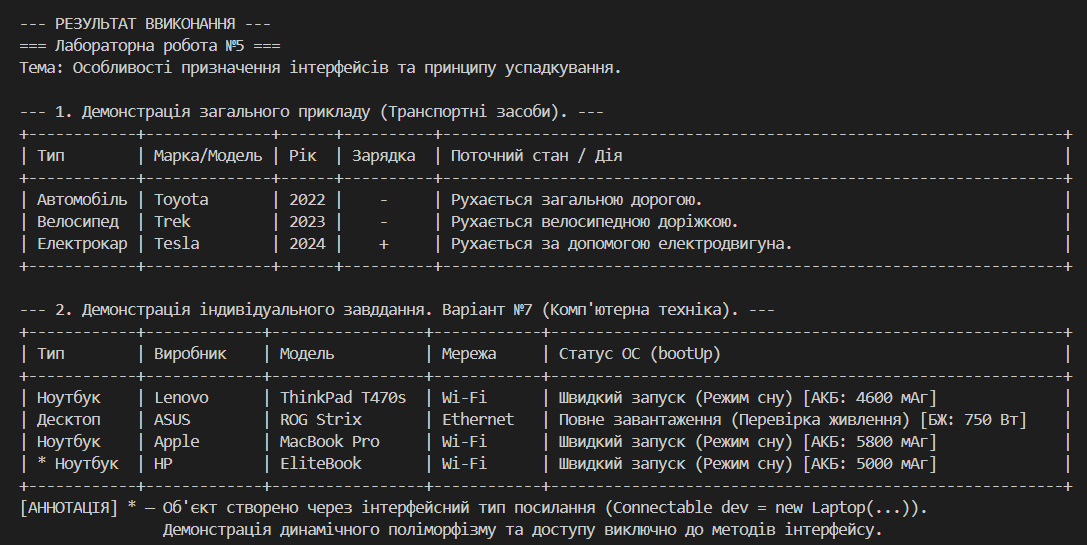
\includegraphics[width=0.95\textwidth]{screenshots/terminal_output.png}
    \caption{Скріншот результатів виконання програми в терміналі VS Code завдання лабораторної роботи №5}
    \label{fig:terminal_output}
\end{figure}

Завдяки винесенню логіки форматування в головний клас \texttt{Main.java} було реалізовано 
принцип розділення відповідальності. Дочірні класи не містять 
елементів CLI-розмітки, повертаючи виключно інформаційні рядки стану, що дозволяє гнучко 
масштабувати систему та змінювати формат представлення даних без рефакторингу бізнес-логіки 
ієрархії.

% Контрольні запитання
\section{Відповіді на контрольні запитання}

\begin{enumerate}
    \item \textbf{Що таке успадкування в об'єктно-орієнтованому програмуванні?}
    Це фундаментальний принцип ООП, який дозволяє створювати новий (дочірній) клас 
    на основі вже існуючого (батьківського), автоматично переймаючи його захищені 
    та публічні поля і методи для повторного використання коду та розширення 
    функціональності.

    \item \textbf{Яке ключове слово використовується для успадкування класів у Java?}
    Для реалізації успадкування класів у мові програмування Java використовується 
    ключове слово \texttt{extends}.

    \item \textbf{Чим відрізняється базовий клас від дочірнього?}
    Базовий (батьківський) клас описує загальні універсальні характеристики сутностей, 
    тоді як дочірній (похідний) клас конкретизує поведінку, додає власні унікальні 
    поля/методи та перевизначає логіку суперкласу.

    \item \textbf{Чи може клас у Java успадковувати декілька класів одночасно?}
    Ні, в Java реалізовано лише поодиноке успадкування для класів (конструкція з 
    кількома батьківськими класами не підтримується), проте один клас може реалізовувати 
    декілька інтерфейсів одночасно.

    \item \textbf{Для чого використовується ключове слово super?}
    Ключове слово \texttt{super} використовується для звернення до елементів батьківського
     класу: для виклику його конструктора на початку конструктора дочірнього класу 
     (наприклад, \texttt{super(brand, model)}) або для виклику оригінальних методів 
     суперкласу.

    \item \textbf{Що таке перевизначення методу?}
    Це операція, за якої дочірній клас змінює внутрішню реалізацію (тіло методу) 
    успадкованого від батьківського класу методу при повному збереженні його імені, 
    аргументів та типу повертаємого значення.

    \item \textbf{Для чого використовується анотація @Override?}
    Вона рекомендується для позначення перевизначеного методу та вказує компілятору Java 
    на перевірку відповідності сигнатур. Це захищає від помилок друку — якщо сигнатури 
    методів базового та дочірнього класів не збігаються, компілятор видасть помилку.

    \item \textbf{Що таке абстрактний клас?}
    Це клас, оголошений із ключовим словом \texttt{abstract}, який призначений для 
    створення спільної основи для інших класів. Він може містити як звичайні методи 
    з реалізацією, так і абстрактні методи без тіла.

    \item \textbf{Чи можна створити безпосередньо об'єкт абстрактного класу?}
    Ні, створити безпосередньо об'єкт абстрактного класу неможливо (наприклад, виклик 
    \texttt{new ComputerDevice()} призведе до помилки компіляції).

    \item \textbf{Що таке абстрактний метод?}
    Це метод, який оголошується без тіла (без конкретної реалізації, завершується 
    крапкою з комою), задаючи лише сигнатуру, яку всі конкретні дочірні класи обов'язково 
    повинні реалізувати.

    \item \textbf{Які елементи може містити абстрактний клас?}
    Абстрактний клас може містити поля (змінні стану), конструктори, звичайні методи з 
    реалізацією, а також абстрактні методи без реалізації.

    \item \textbf{Що таке інтерфейс у Java?}
    Це повністю абстрактна конструкція, створена за допомогою ключового слова 
    \texttt{interface}, яка визначає певний набір методів (контракт поведінки), що повинні 
    бути реалізовані класом.

    \item \textbf{Яке ключове слово використовується для реалізації інтерфейсу?}
    Клас реалізує інтерфейс за допомогою ключового слова \texttt{implements}.

    \item \textbf{Чи може один клас реалізовувати декілька інтерфейсів?}
    Так, однією з важливих переваг інтерфейсів є можливість реалізувати декілька інтерфейсів 
    одним конкретним класом через кому.

    \item \textbf{У чому полягає основна відмінність між абстрактним класом та інтерфейсом?}
    Абстрактний клас доцільно використовувати тоді, коли класи мають спільний стан, поля та 
    частково спільну реалізацію (зв'язок сутностей). Інтерфейс доцільно використовувати для 
    визначення певної можливості або набору операцій, які можуть бути реалізовані різними, 
    навіть не пов'язаними між собою класами.

    \item \textbf{Що таке поліморфізм?}
    Це принцип ООП, який дає змогу працювати з об'єктами різних дочірніх класів через 
    спільний базовий тип (суперклас або інтерфейс), забезпечуючи виконання потрібної 
    реалізації методу на етапі виконання програми.

    \item \textbf{Для чого можна використовувати інтерфейс як тип змінної?}
    Це дозволяє створювати універсальний, гнучкий код, який абстрагується від конкретних 
    класів у кучі (Heap) та працює з усіма об'єктами, що реалізують відповідний інтерфейсний 
    контракт (наприклад, \texttt{Connectable officeLaptop = new Laptop(...)}).

    \item \textbf{Що відбувається під час виклику перевизначеного методу через змінну базового типу?}
    Завдяки механізму динамічного поліморфізму, під час виконання програми віртуальна машина 
    Java (JVM) аналізує фактичний тип об'єкта, на який посилається змінна, і викликає саме 
    перевизначену реалізацію дочірнього класу.

    \item \textbf{Для чого в об'єктно-орієнтованому програмуванні використовують абстракцію?}
    Для виділення головних, спільних та визначальних характеристик об'єктів певної предметної 
    області й відсікання другорядних деталей реалізації, що допомагає проектувати архітектуру 
    складних систем.

    \item \textbf{Які переваги дає використання успадкування та інтерфейсів під час розроблення програм?}
    Успадкування дозволяє уникати дублювання коду та будувати чіткі ієрархії пов'язаних класів, 
    а інтерфейси дозволяють визначати спільні гнучкі правила взаємодії між різними класами, 
    забезпечуючи легкість розширення та масштабування програми.
\end{enumerate}

% Інформаційні ресурси та посилання на вихідний код
\section{Інформаційні ресурси та посилання на вихідний код}

Згідно з вимогами до здачі лабораторної роботи, повний проект розробленого вихідного коду   
додатку, розміщено у віддаленому репозиторії системи контролю версій. 

\begin{itemize}
    \item \textbf{Посилання на Git-репозиторій проєкту:} \\
    \texttt{https://github.com/nasuehfw/oop-lab5.git} % TODO: Тут моя реальная ссылка на github!
    \item \textbf{Електронний каталог спільного доступу:} \\
    % Обновленна ссылка после трабола на моем диске
    \url{https://drive.google.com/drive/folders/1oiJNrP62_ZFaXsxSDoPd4y1sXu0Bt5s1?usp=drive_link} 
\end{itemize}



% Литератупа
%\makebibliography
%\input{sections/literature.tex}

% Аппендикс (если нужен)
%\appendix
%\input{appendix/appendix.tex}


\end{document}
